% Mighty Maps -- Geospatial Visualization with Google Earth and KML
\documentclass{beamer}
\usetheme{Madrid}
\usefonttheme{serif}
\usefonttheme{structuresmallcapsserif}
\usepackage{fancyvrb}

\newenvironment<>{varblock}[2][\textwidth]{
    \begin{center}
        \begin{minipage}{#1}
            \setlength{\textwidth}{#1}
            \begin{actionenv}#3
                \def\insertblocktitle{#2}
                \par
                \usebeamertemplate{block begin}}
            {\par
                \usebeamertemplate{block end}
            \end{actionenv}
        \end{minipage}
    \end{center}
}

\begin{document}

\title{Mighty Maps}
\subtitle{Geospatial Visualization with Google Earth and KML}
\author{Joshua Tolley}
\institute{End Point Corp.}

\frame{\titlepage}

\begin{frame}{Cool Kids Do Data Visualization}
    \begin{columns}[c]
        \column{0.3\textwidth}
        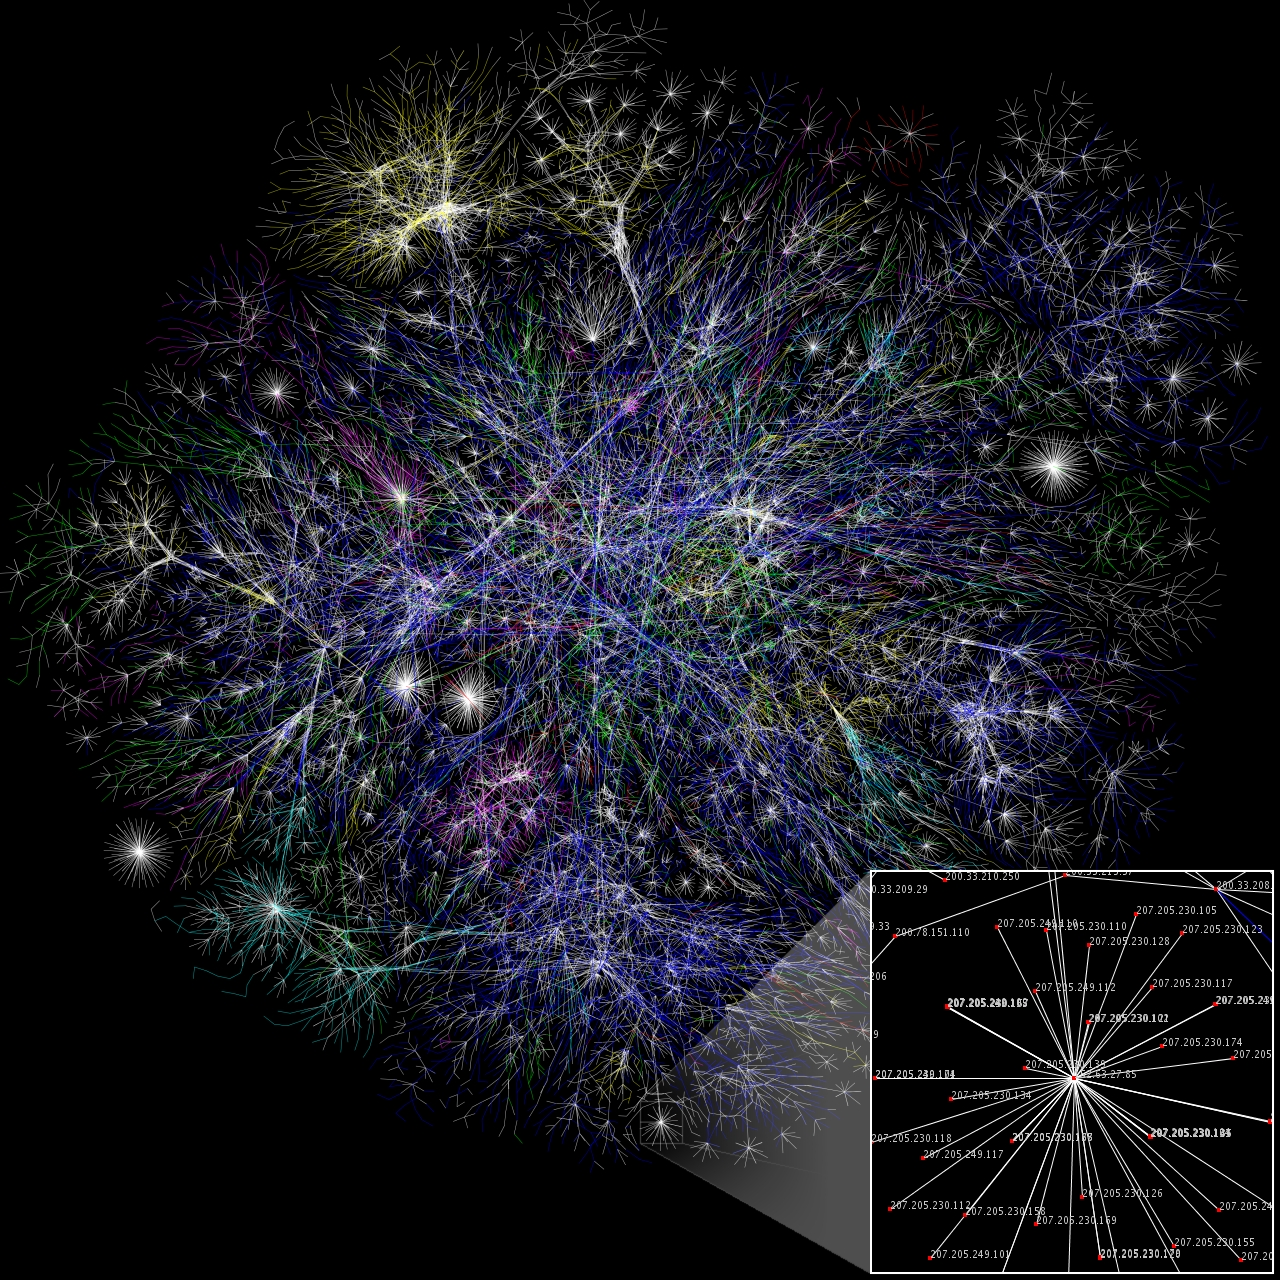
\includegraphics[width=\textwidth]{Internet_map_1024.jpg}
        \\
        {\small The Opte Project}

        \column{0.6\textwidth}
        Everyone seems to have data, and lots of it. Everyone seems to want pictures of their data.
    \end{columns}
\end{frame}

\begin{frame}{Cool Kids Do Data Visualization}
    \begin{columns}[c]
        \column{0.3\textwidth}
        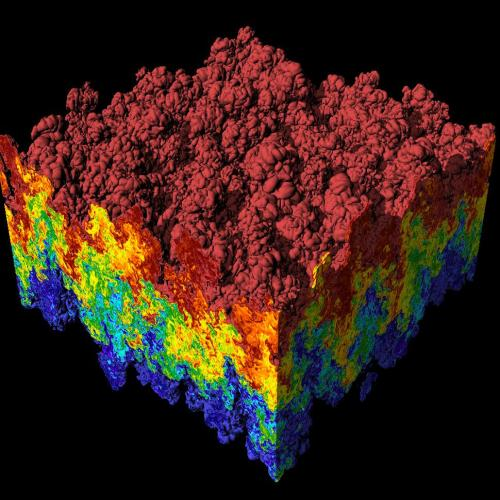
\includegraphics[width=\textwidth]{Rayleigh-Taylor_instability.jpg}
        \\
        {\small Lawrence Livermore National Laboratory}

        \column{0.6\textwidth}
        Visualization has become a vibrant field of study. People blog about visualizations.
    \end{columns}
\end{frame}

\begin{frame}{Cool Kids Do Data Visualization}
    In particular, people love geospatial visualization. Perhaps because
    everyone has geographic data, and Google's Maps API is easy.
    \begin{center}
        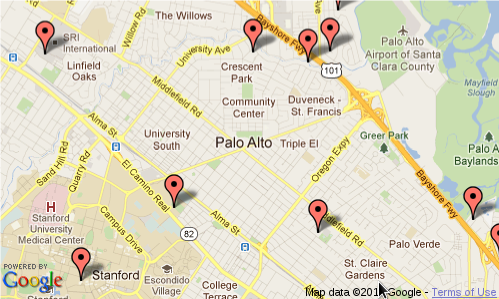
\includegraphics[width=0.8\textwidth]{Maps_API.png}
    \end{center}
\end{frame}

\begin{frame}{Cool Kids Do Data Visualization}
    \begin{center}
        ...or other APIs, if you prefer...
        \\
        \vspace{0.1\textheight}
        
\includegraphics[width=0.8\textwidth]{mapping_apis.png}
    \end{center}
\end{frame}

\begin{frame}{Geospatial Visualization}
    Geospatial visualization is \ldots
    \begin{itemize}
        \item It's easy to understand, compared to dots and lines. Everyone understands maps
        \item The selection of APIs makes it easy to do
        \item Everyone has geographic data
        \begin{itemize}
            \item Who browsed my website, from where? (GeoIP)
            \item Where do I ship most of my orders
            \item What, in fact, are the migration patterns of African and European swallows?
        \end{itemize}
    \end{itemize}
\end{frame}

\begin{frame}{Everyone has Geographic Data}
    \begin{varblock}[0.9\textwidth]{Note}
        Although everyone has geographic data, it's not necessarily important data.
    \end{varblock}
\end{frame}

\begin{frame}{Everyone has Geographic Data}
    \begin{varblock}[0.9\textwidth]{Note}
        The fact that particular data are unimportant or even meaningless rarely prevents people from trying to make a picture out of them.
    \end{varblock}
\end{frame}

\frame{There are some cool things happening in geovisualization\ldots}

\begin{frame}{Google Earth}
    Google Earth is essentially Google Maps in 3D.
    \begin{center}
        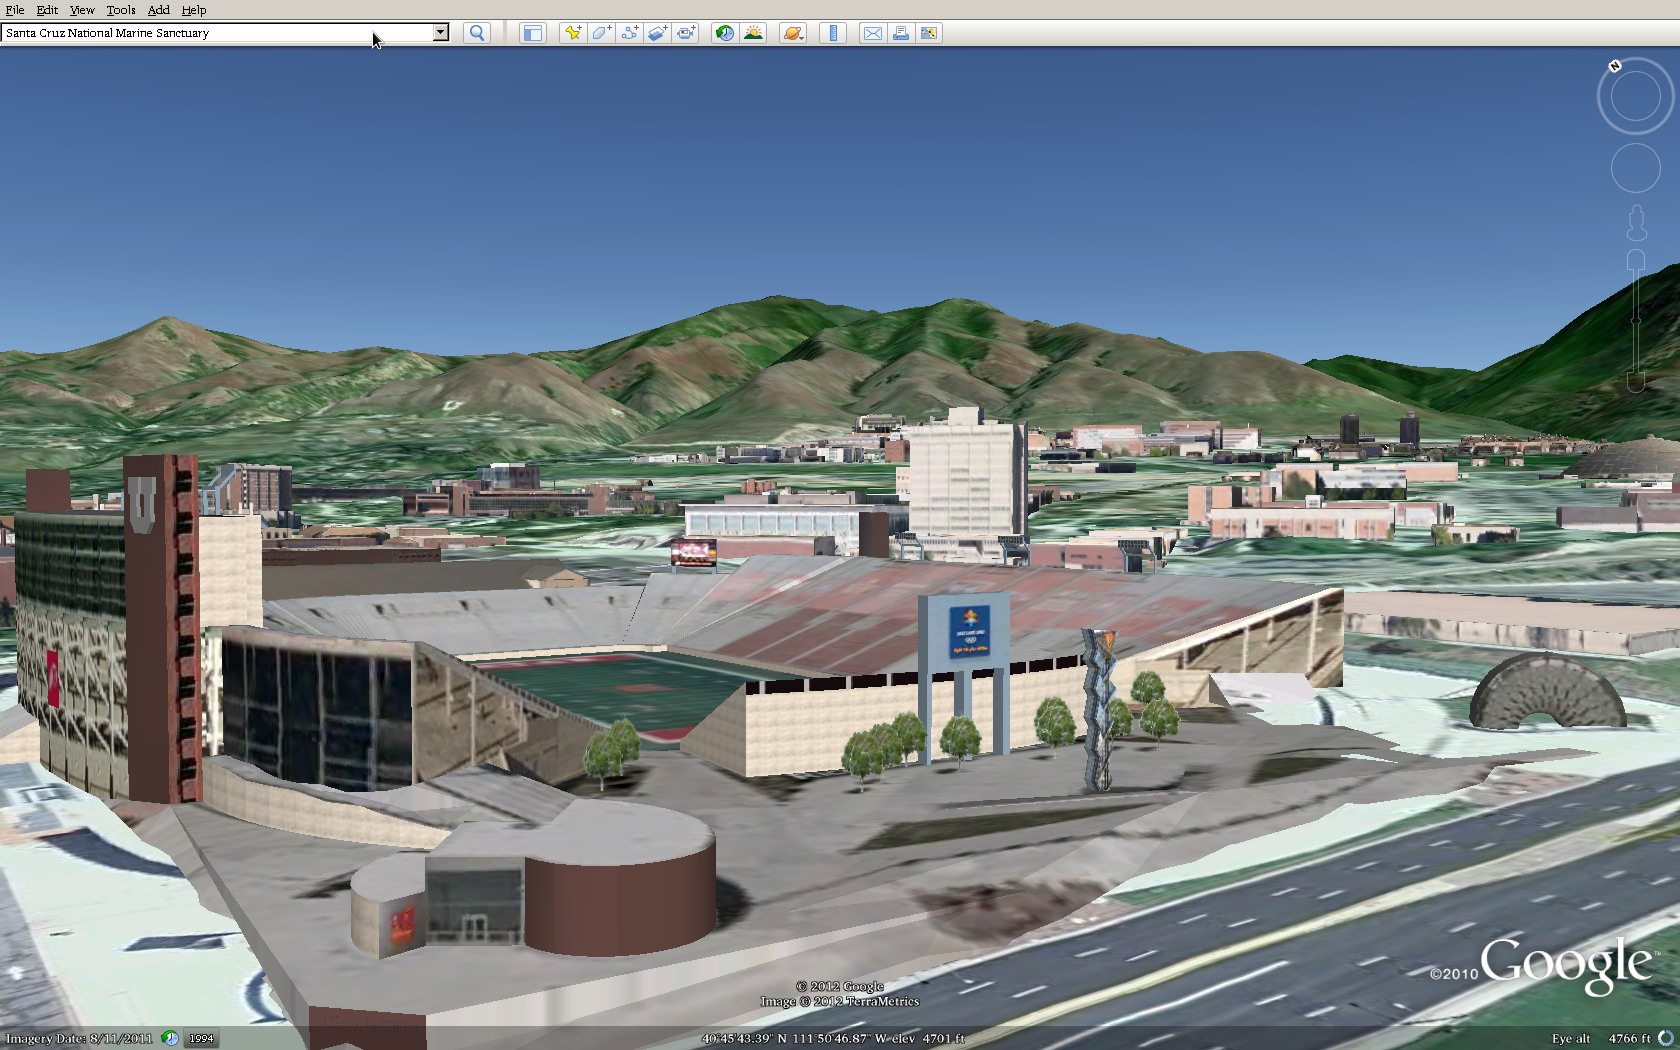
\includegraphics[width=0.8\textwidth]{RiceEcclesStadium.png}
    \end{center}
\end{frame}

\begin{frame}{What's Google Earth?}
    \begin{itemize}
        \item Desktop application for Linux (and Mac and Windows, if you insist)
        \item Free, but not open source ;(
        \item There exists a paid ``professional'' version
        \begin{itemize}
            \item Allows rendering of video, more flexible editing of large data sets, and a few other things
        \end{itemize}
        \item Also exists in browser plugin form with JavaScript control; this works only on Mac and Windows
        \item Began as a project by Keyhole software, which Google eventually bought
    \end{itemize}
\end{frame}

\begin{frame}{How to use Google Earth}
    Google Earth accepts files written in Keyhole Markup Language
    \begin{itemize}
        \item XML-based
        \item Can be created automatically through Google Earth; IMO this is not terribly flexible
        \item Can be written by hand; IMO this is like chewing glass
        \item Can be generated by various helper projects
        \begin{itemize}
            \item Kamelopard: Ruby-based. I wrote it, and use it a lot.
            \item PyKML: Python-based. More polished and consistent, but seemingly less capable than Kamelopard
        \end{itemize}
    \end{itemize}
\end{frame}

\begin{frame}{Aside}
    This presentation won't show you much KML. Its point is to show some of what can be done, leaving the KML as an exercise for the reader.
\end{frame}

\begin{frame}{An Example}
    I live on a small farm, where we are growing 12 acres of wheat and raising various poultry. It's here. This is a KML Placemark.
    \begin{center}
        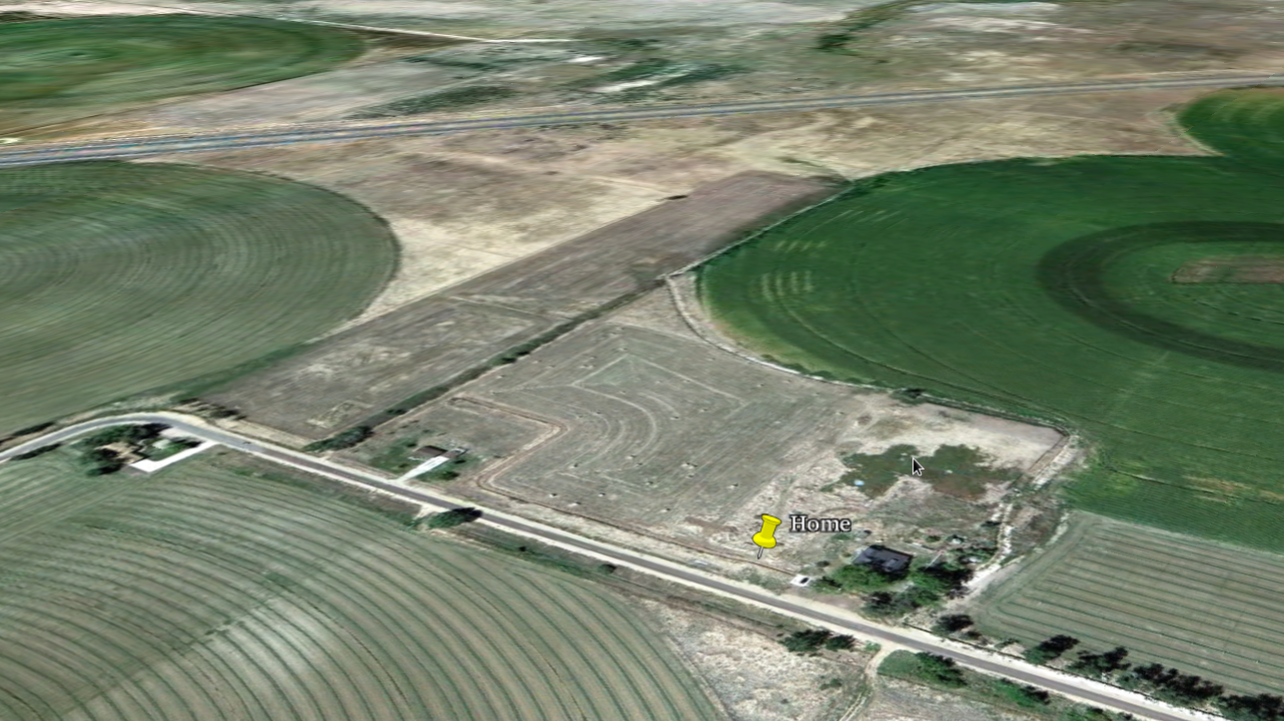
\includegraphics[width=0.8\textwidth]{home-1.png}
    \end{center}
\end{frame}

\begin{frame}{An Example}
    These placemarks have descriptions, which can pop up in balloons, like this one. This can include CSS, images, or even Flash video. Icons, text, and balloons can all be styled at will.
    \begin{center}
        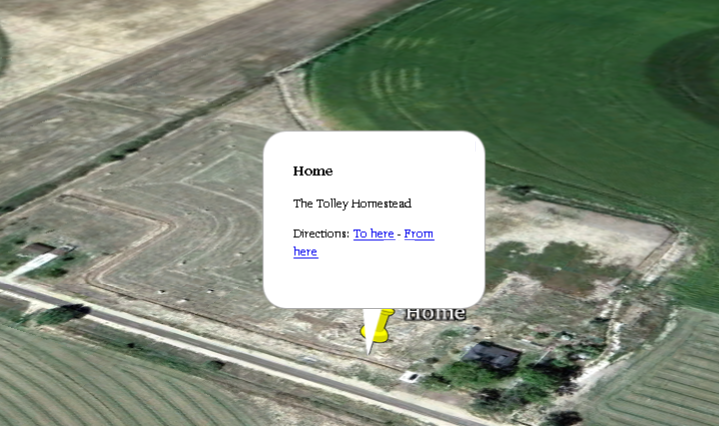
\includegraphics[width=0.8\textwidth]{home-2.png}
    \end{center}
\end{frame}

\begin{frame}{An Example}
    As I said, we're growing wheat this year. This shows the wheat field, outlined with a KML polygon. KML also allows other objects, like lines and 3D models, in various styles.
    \begin{center}
        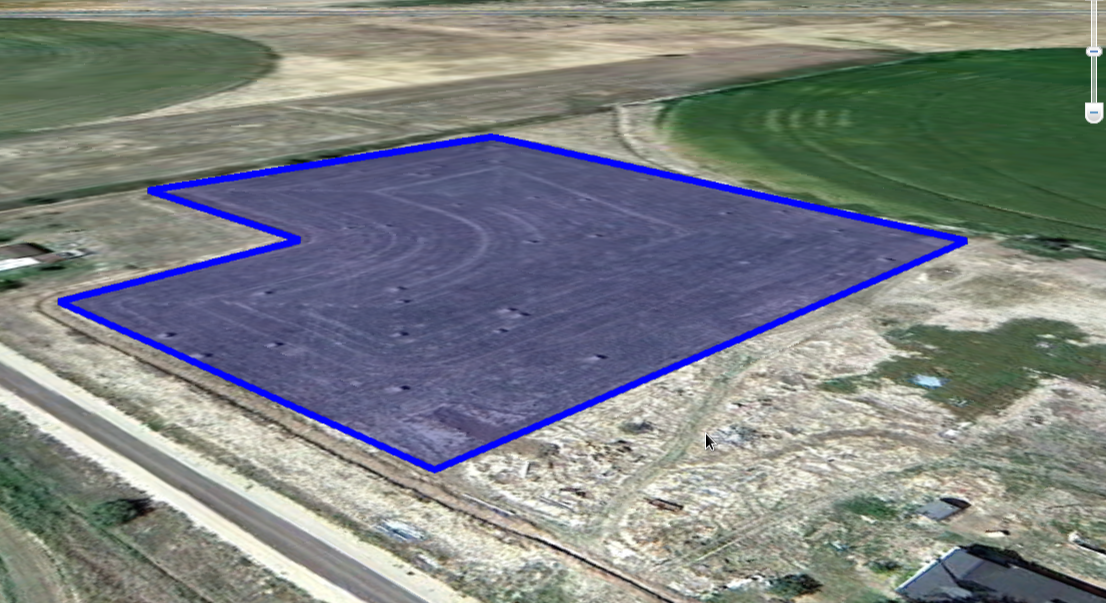
\includegraphics[width=0.8\textwidth]{wheat.png}
    \end{center}
\end{frame}

\begin{frame}{An Example}
    Some of these KML objects can include time data
    \begin{center}
        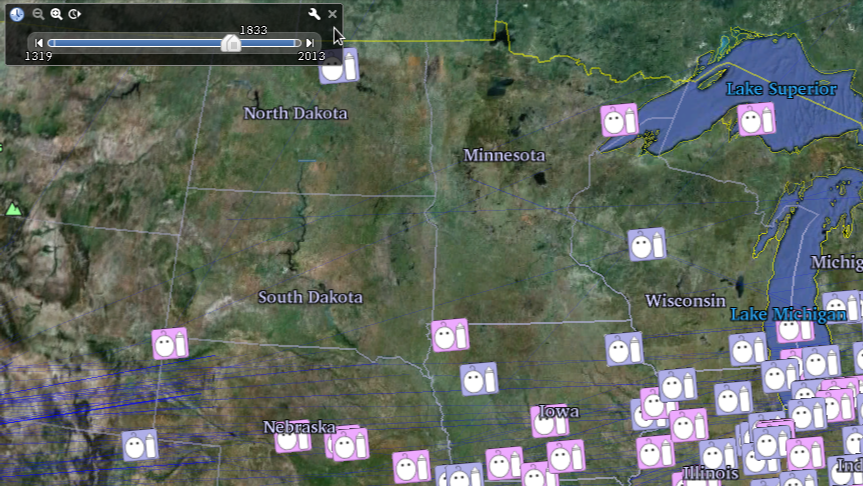
\includegraphics[width=0.8\textwidth]{history.png}
    \end{center}
\end{frame}

\begin{frame}{An Example}
    Google Earth allows a few different kinds of added images in a scene,
    called ``Overlays''. This is a Screen Overlay.
    \begin{center}
        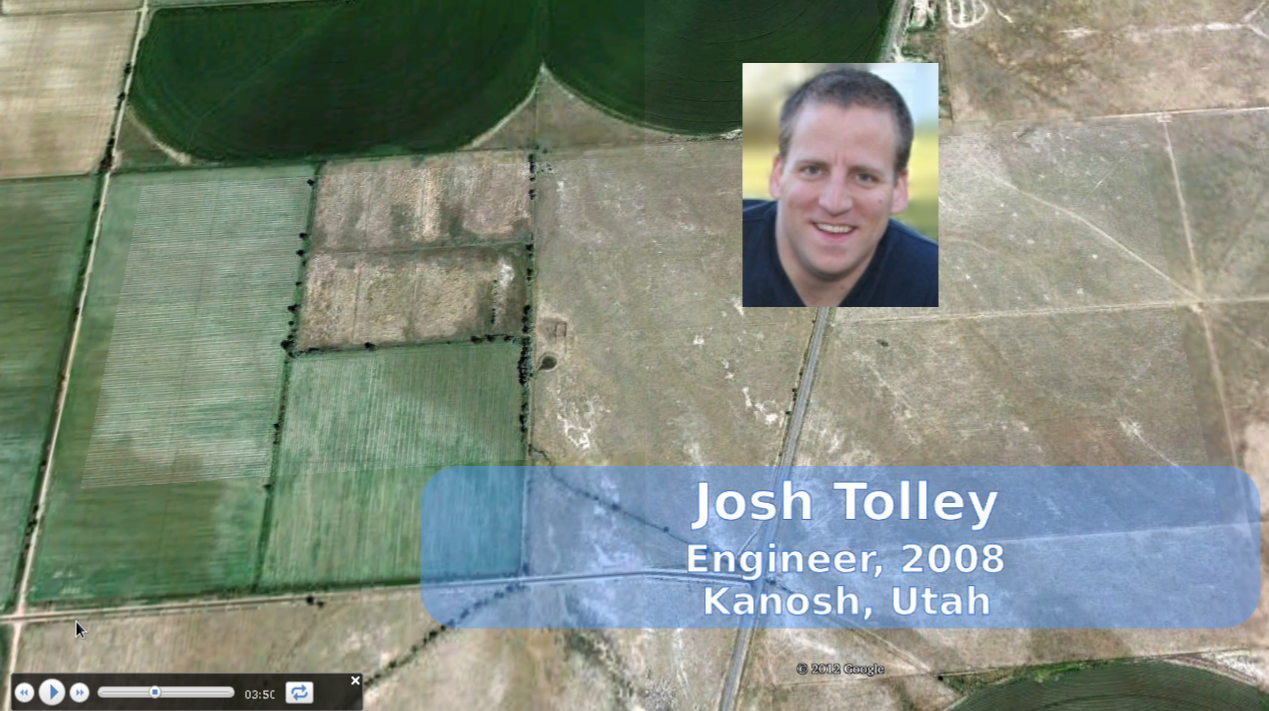
\includegraphics[width=0.8\textwidth]{screenoverlay.png}
    \end{center}
\end{frame}

\begin{frame}{An Example}
    Images, placemarks, overlays, etc. call be grouped and animated in a ``Tour''
    \begin{center}
        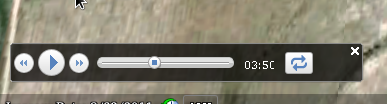
\includegraphics[width=0.8\textwidth]{tourcontrol.png}
    \end{center}
    Tours navigate the viewer automatically, displaying and hiding objects at
    precise locations and for well-defined durations. They can include
    background audio.
\end{frame}

\begin{frame}{Liquid Galaxy}
    Google Earth can talk to itself, to broadcast its view of the world. It can
    also receive these packets, and show related views. So if you put multiple
    instances together, you get a panoramic view. This is called a Liquid
    Galaxy.
    \begin{center}
        % XXX insert image of liquid galaxy here
        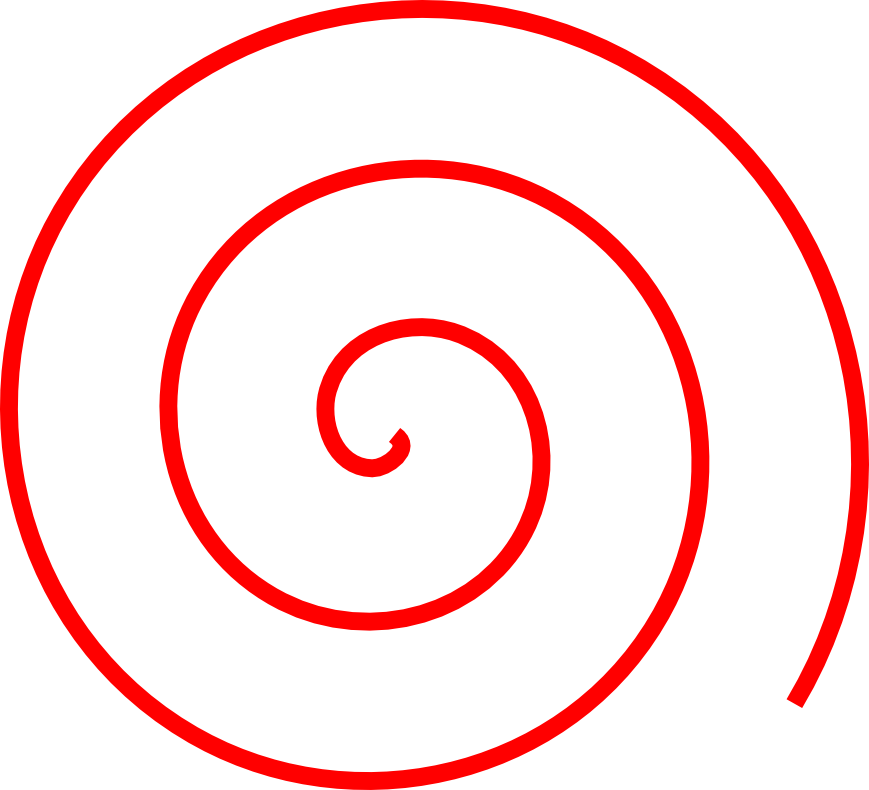
\includegraphics[width=0.8\textwidth]{spiral.png}
    \end{center}
\end{frame}

\begin{frame}{Liquid Galaxy}
    End Point has done lots of work with Liquid Galaxies:
    \begin{itemize}
        \item They boot custom ISOs from a network
        \item Tours and content can be controlled via touch screen
        \item Techs can monitor and repair galaxies remotely, easily
        \item Tour content seamlessly integrates Google Earth with other applications, such as mplayer
        \item It's all open source
    \end{itemize}
    Come see our booth :)
\end{frame}

\begin{frame}{Making tours}
    \begin{varblock}[0.9\textwidth]{Universal Truth}
        Writing XML in significant quantities by hand sucks. Debugging and modifying it later sucks worse.
    \end{varblock}
\end{frame}

\begin{frame}{Making tours}
    \begin{columns}[c]
        \column{0.3\textwidth}
        % XXX include giraffe image here
        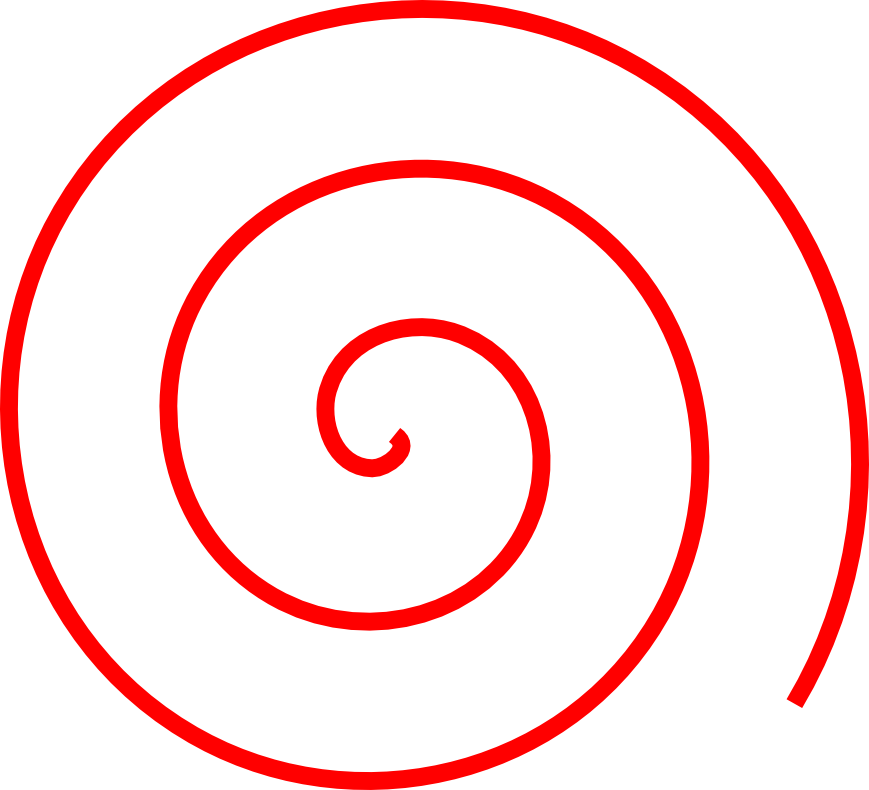
\includegraphics[width=\textwidth]{spiral.png}

        \column{0.6\textwidth}
        Enter ``Kamelopard'':
        \begin{itemize}
            \item Writes KML for you
            \item Ruby-based, for buzzword appeal
            \item Open source, so you can fix what's broken
            \item Awkward name. It worked for PostgreSQL...
        \end{itemize}
    \end{columns}
\end{frame}

\begin{frame}[fragile]
    \frametitle{Making tours}
    \begin{Verbatim}[fontfamily=courier]
  require 'rubygems'
  require 'kamelopard'
  require 'yaml'

  f = Kamelopard::Folder.new 'Tour Resources'
  data = YAML::load_file 'some_data.yml'
  data.each do |d|
    p = point d[:longitude], d[:latitude]
    pl = Kamelopard::Placemark p, :desc => d[:desc]
    f << pl
  end

  write_kml_to 'doc.kml'
    \end{Verbatim}
\end{frame}

% XXX Insert sample of more interesting Kamelopard code

\begin{frame}{Kamelopard}
    Kamelopard makes it easy (and succinct!) to generate KML for large data sets, using complicated algorithms.
    \begin{itemize}
        \item Tour of End Point employees, taken straight from employee database
        \item FamilySearch mashup; show ancestral migrations
        \item ``Smart'' power meters' trouble messages vs. lightning strikes
        \item Fisheries' catch records plotted historically, also straight from the database
    \end{itemize}
\end{frame}

\end{document}
